% \item \textbf{\cref{fig:introduction:ai-products} (p\pageref{fig:introduction:ai-products})}
%   is a reproduction of \citet{LoGiudice:2016wf}'s report on how \gls{ai} will re-shape applications. The authors produce three primary categories and list sample products, vendors and use cases. This image was originally included within \cref{ch:background}.
% \item \textbf{\cref{fig:introduction:stackoverflow-trends} (p\pageref{fig:introduction:stackoverflow-trends})}

\section{Motivating Scenarios}
\label{ssec:introduction:motivation}

The market for \glsplx{cvs} is expanding (\cref{tab:introduction:ai-products}) with a corresponding interest from developers (\cref{fig:introduction:stackoverflow-trends}). These services are inherently probabilistic in their behaviour, in that the end-points always return with a response with a probability. This is unlike a typical \gls{api} that would return a response (\textit{without} a probability) or an error.  If developers do not fully understand the nature of these services when integrating with them, there is an impact on the quality of software they create.

To illustrate the context of use, we present the two scenarios of varying risk: (i)~a fictional software developer, named Tom, who wishes to develop an inherently low-risk photo labelling application for his friends and family; and (ii) a high-risk cancer \gls{cdss} that uses patient scans to recommend if surgeons should send their patients to surgery. Both describe scenarios where \gls{ai}-infused components has an impact to end-users when the software engineers developing with them misunderstand the nuances of \gls{ml}, ultimately affecting external quality. Moreover, when developers lack a comprehension, this hinders their productivity and understanding/appreciation of \gls{ai}-based components.
  
\subsection{Low Risk Motivating Scenario}
\label{ssec:introduction:motivation:scenario:pam}

Tom wants to develop a social media photo-sharing app on iOS and Android, \textit{PhotoSharer}, that analyses photos taken on smartphones. Tom wants the app to categorise photos into scenes (e.g., day vs. night, landscape vs. indoors), generate brief descriptions of each photo, and catalogue photos of his friends and common objects (e.g., photos with his Border Collie dog, photos taken on a beach on a sunny day with his partner). His app will shares this analysed photo intelligence with his friends on a social-media platform, where his friends can search and view the photos.

Instead of building a computer vision engine from scratch, which takes too much time and effort, Tom thinks he can achieve this using one of the common \glspl{cvs}. Tom comes from a typical software engineering background and has insufficient knowledge of key computer vision terminology and no understanding of its underlying techniques. However, inspired by easily accessible cloud \glspl{api} that offer computer vision analysis, he chooses to use these. Built upon his experience of using other similar cloud services, he decides on one of the \gls{cvs} \glspl{api}, and expects a static result always and consistency between similar \glspl{api}. Analogously, when Tom invokes the iOS Swift substring method \texttt{"doggy".prefix(3)}, he expects it to be consistent with the Android Java equivalent \texttt{"doggy".substring(0, 2)}. Consistent, here, means two things: (i) that calling \texttt{substring} or \texttt{prefix} on \texttt{`dog'} will \textit{always} return in the same way every time he invokes the method; and (ii) that the result is \textit{always} \texttt{`dog'} regardless of the programming language or string library used, given the deterministic nature of the `substring' construct (i.e., results for substring are \gls{api}-agnostic). 

\begin{table}[th!]
  \centering
  \caption[Varying confidence changes over time between 3 CV APIs]{First six responses of image analysis for a Border Collie sent to three computer vision \gls{cis} \glspl{api} providers five months apart. The specificity (to 3 s.f.) and vocabulary of each label in the response varies between all services, and---except for Provider B---changes over time. Any confidence changes greater than 1 per cent are highlighted in red.}
  \label{tab:introduction:motivation:scenario:pam:confchanges}
  \begin{tabular}{l|c|c|c|c|c|c}
    \toprule
    \multirow{2}{*}{\bfseries Label} &
    \multicolumn{2}{c}{\bfseries Provider A} &
    \multicolumn{2}{c}{\bfseries Provider B} &
    \multicolumn{2}{c}{\bfseries Provider C} \\
    &
    Aug 2018 & Jan 2019 &
    Aug 2018 & Jan 2019 &
    Aug 2018 & Jan 2019 \\
    \midrule
    Dog             & 0.990 & \textcolor{red}{0.986} & 0.999 & 0.999 & 0.992 & \textcolor{red}{0.970} \\
    Dog Like Mammal & 0.960 & 0.962 & -     & -     & -     & -     \\
    Dog Breed       & 0.940 & 0.943 & -     & -     & -     & -     \\
    Border Collie   & 0.850 & 0.852 & -     & -     & -     & -     \\
    Dog Breed Group & 0.810	& 0.811 & -     & -     & -     & -     \\
    Carnivoran      & 0.810 & \textcolor{red}{0.680} & -     & -     & -     & -     \\
    Black           & -     & -     & 0.992 & 0.992 & -     & -     \\
    Indoor          & -     & -     & 0.965 & 0.965 & -     & -     \\
    Standing        & -     & -     & 0.792 & 0.792 & -     & -     \\
    Mammal          & -     & -     & 0.929 & 0.929 & 0.992 & \textcolor{red}{0.970} \\
    Animal          & -     & -     & 0.932 & 0.932 & 0.992 & \textcolor{red}{0.970} \\
    Canine          & -     & -     & -     & -     & 0.992 & \textcolor{red}{0.970} \\
    Collie          & -     & -     & -     & -     & 0.992 & \textcolor{red}{0.970} \\
    Pet             & -     & -     & -     & -     & 0.992 & \textcolor{red}{0.970} \\
    \bottomrule
  \end{tabular}
\end{table}

More concretely, in \cref{tab:introduction:motivation:scenario:pam:confchanges}, we illustrate how three (anonymised) \gls{cvs} providers fail to provide similar consistency to that of the substring example above. If Tom uploads a photo of a border collie\footnote{The image used for these results is \url{https://www.akc.org/dog-breeds/border-collie/}.} to three different providers in August 2018 and January 2019, he would find that each provider is different in both the vocabulary used between. The confidence values and labels within the \textit{same} provider varies within a matter of five months. The evolution of the confidence changes is not explicitly documented by the providers (i.e., when the models change) nor do they document what confidence means. Service providers use a tautological nature when defining what the confidence values are (as presented in the \gls{api} documentation) provides no insight for Tom to understand why there was a change in confidence, which we show in \cref{tab:introduction:motivation:scenario:pam:tautological}, unless he \textit{knows} that the underlying models change with them. Furthemore, they do not provide detailed understanding on how to select a threshold cut-off for a confidence value. Therefore, he's left with no understanding on how best to tune for image classification in this instance. The deterministic problem of a substring compared to the nondeterministic nature of the \gls{iws} is, therefore, non-trivial.

\begin{table}[hbt]
  \centering
  \caption[Tautological definitions of confidence found in API documentation]{Tautological definitions of `confidence' found in the \gls{api} documentation of three common \gls{cvcis} providers.}
  \label{tab:introduction:motivation:scenario:pam:tautological}
  \begin{tabular}{l|p{0.8\linewidth}}
    \toprule
    \bfseries \gls{api} Provider &
    \bfseries Definition(s) of Confidence \\
    \midrule
    Provider A &
      \itshape  
      ``Score is the confidence score, which ranges from 0 (no confidence) to 1 (very high confidence).''
      \upshape
      \citepweb{Google:ConfidenceScore_DocsLabel}
      \bigskip
      
      \itshape  
      ``Deprecated. Use score instead. The accuracy of the entity detection in an image. For example, for an image in which the `Eiffel Tower' entity is detected, this field represents the confidence that there is a tower in the query image. Range [0, 1].'' 
      \upshape
      \citepweb{Google:ConfidenceScore_DotNet} 
      \bigskip
      
      \itshape  
      ``The overall score of the result. Range [0, 1]''
      \upshape
      \citepweb{Google:ConfidenceScore_DotNet} 
      \bigskip
    \\ 
    Provider B &
      \itshape  
        ``Confidence score, between 0 and 1... if there insufficient confidence in the ability to produce a caption, the tags maybe [sic] the only information available to the caller.''
      \upshape
      \citepweb{Azure:ConfidenceScore_HowToCall}
      \bigskip
      
      \itshape  
        ``The level of confidence the service has in the caption.''
      \upshape
      \citepweb{Azure:ConfidenceScore_JavaDocs}    
      \bigskip
    \\
    Provider C &
      \itshape  
        ``The response shows that the operation detected five labels (that is, beacon, building, lighthouse, rock, and sea). Each label has an associated level of confidence. For example, the detection algorithm is 98.4629\% confident that the image contains a building.''
      \upshape
      \citepweb{AWS:ConfidenceScore_DetectLabel}
      \bigskip
      
      \itshape  
        ``[Provider C] also provide[s] a percentage score for how much confidence [Provider C] has in the accuracy of each detected label.''
      \upshape
      \citepweb{AWS:ConfidenceScore_DetectObjScene}
    \\
    \bottomrule
  \end{tabular}
\end{table}


To make an assessment of these \glspl{api}, he tries his best to read through the documentation of different \gls{cvs} \glspl{api}, but he has no guiding framework to help him choose the right one. A number of questions come to mind:

\begin{itemize}
  \item What does `confidence' mean?%ICSME(?) \todo {did this change to score in the new versions?}
  \item Which confidence is acceptable in this scenario?%fse-demo
  \item Are these \glspl{api} consistent in how they respond?%ICSME
  \item Are the responses in \glspl{api} static and deterministic?%ICSME
  \item Would a combination of multiple \gls{cvs} \glspl{api} improve the response?%ICWE
  \item How does he know when there is a defect in the response? How can he report it?%ICSE
  \item How does he know what labels the \gls{api} knows, and what labels it doesn't?%ICSE
  \item How does it describe his photos and detect the faces?%ICSE
  \item Does he understand that the \gls{api} uses a machine learnt model? Does he know what a \gls{ml} model is?%ICSE
  \item Does he know when models update? What is the release cycle?%FSE
\end{itemize}

Although Tom generally anticipates these \glspl{cvs} to not be perfect, he has no prior benchmark to guide him on what to expect. The imperfections appear to be low-risk, but may become socially awkward when in use; for instance, if Tom's friends have low self-esteem and use the app, they may be sensitive to the app not identifying them or mislabelling them. Privacy issues come into play especially if certain friends have access to certain photos that they are (supposedly) in; e.g., photos from a holiday with Tom and his partner, however if the \gls{api} identifies Tom's partner as a work colleague, Tom's partner's privacy is at risk.

Therefore, the level of risk and the determination of what constitutes an `error' is dependent on the situation. In the following example, an error caused by the service may be more dangerous.

% Motiviating Example 2: Google Cancer Detect API...

\subsection{High Risk Motivating Scenario}
\label{ssec:introduction:motivation:scenario:cancer}

Recent studies in the oncology domain have used deep-learning \glspl{cnn} to detect \glspl{roi} in image scans of tissue (e.g., \citep{Liu:2018fa,Haenssle:2018bz,EhteshamiBejnordi:2017kq}), flagging these regions for doctors to review. Trials of such algorithms have been able to accurately detect cancer at higher rates than humans, and thus incorporating such capabilities into a \gls{cdss} is closer within reach.  Studies have suggested these systems may erode a practitioner's independent decision-making \citep{Jaspers:2011hy,Chambers:1991uh} due to over-reliance; therefore the risks in developing \glspl{cdss} powered by \glspl{iws} become paramount.

In \cref{fig:introduction:motivation:scenario:cancer} we present a context diagram for a fictional \gls{cdss} named \textit{CancerAssist}. A team of busy pathologists utilise CancerAssist to review patient lymph node scans and discuss and recommend, on consensus, if the patient requires an operation. When the team makes a consensus, the lead pathologist enters the verdict into CancerAssist---running passively in the background---to ensure there is no oversight in the team's discussions. When a conflict exists between the team's verdict and CancerAssist's verdict, the system produces the scan with \glspl{roi} it thinks the team should review. Where the team overrides the output of CancerAssist, this reinforces CancerAssist's internal model as a \gls{hitl} learning process.

\begin{figure}[th]
\centering
  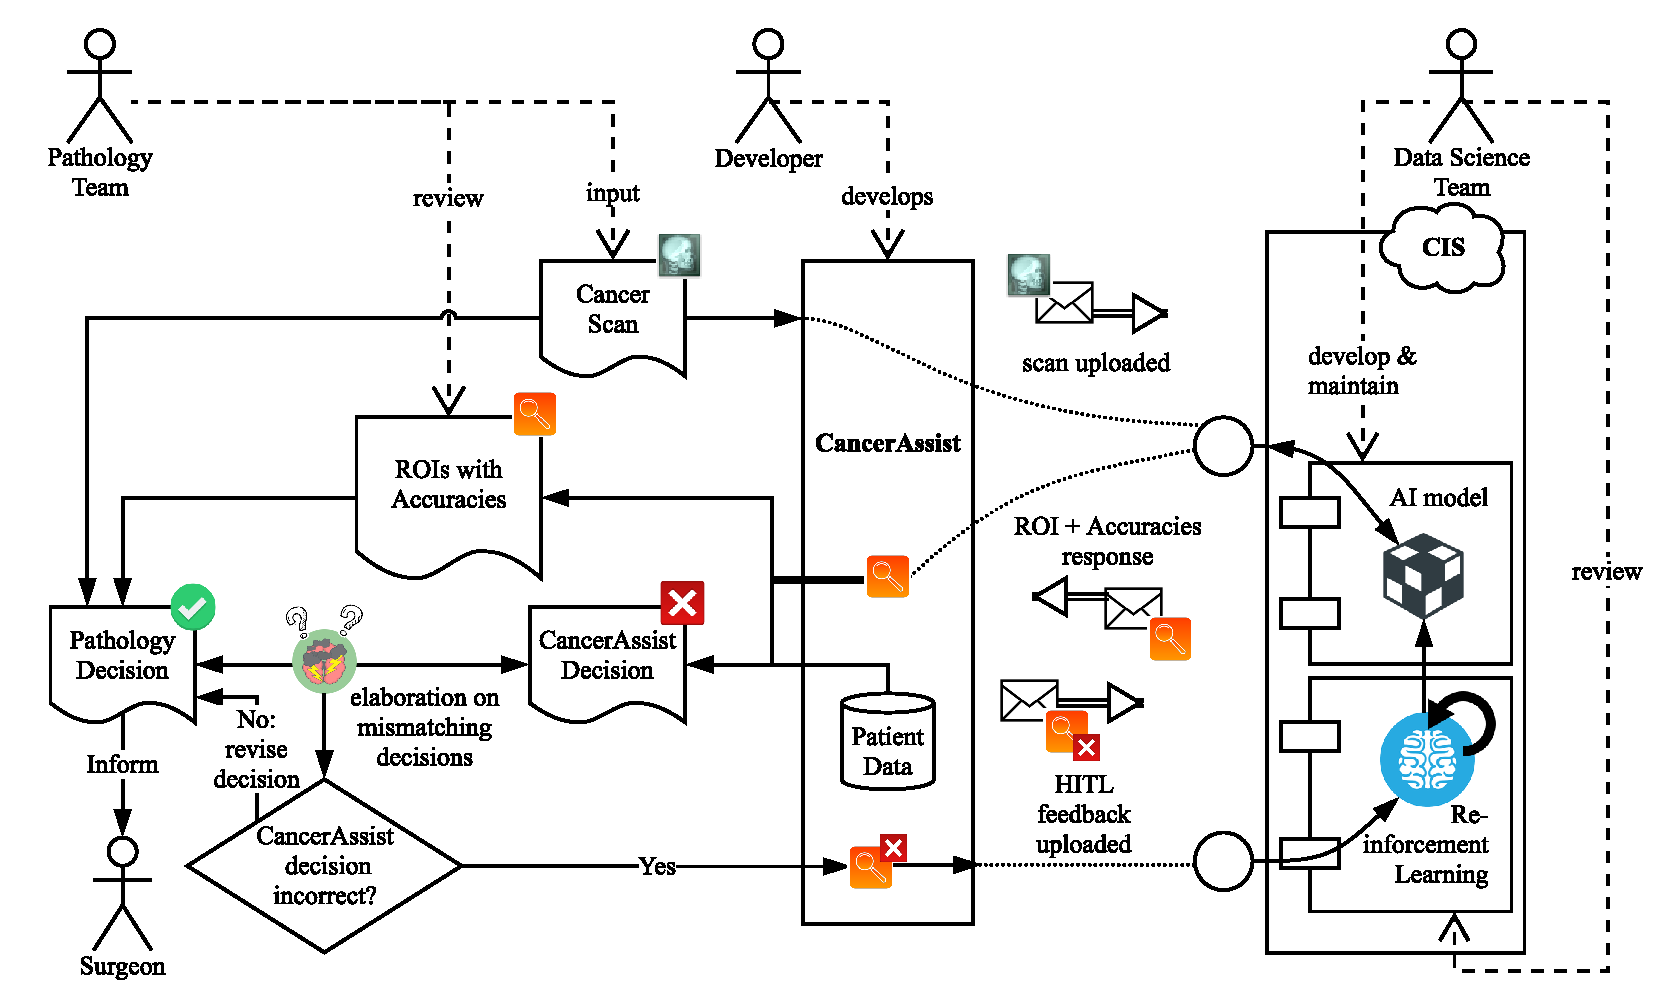
\includegraphics[width=0.8\linewidth]{cancer-assist}
  \caption[CancerAssist Context Diagram]{CancerAssist Context Diagram. \textit{\textbf{Key:} Red Arrows~=~Scan Input; Yellow Arrows~=~Decision Output; Blue Arrows~=~\gls{hitl} Feedback Input.}}
  \label{fig:introduction:motivation:scenario:cancer}
\end{figure}

Powering CancerAssist is Google AI's Lymph Node Assistant (LYNA) \citep{Liu:2018fa}, a \gls{cnn} based on the Inception-v3 model \citep{Szegedy:2016ws,Krizhevsky:2012wl}. To provide intelligence to CancerAssist, the development team decide to host LYNA as an \gls{iws} using a cloud-based \gls{paas} solution. Thus, CancerAssist provides \gls{api} endpoints integrated with patient data and medical history, which produces the verdict. In the case of a positive verdict, CancerAssist highlights the relevant \glspl{roi} found are with their respective bounding boxes and their respective cancer detection accuracies.

The developer of CancerAssist has no interaction with the Data Science team maintaining the LYNA \gls{iws}. As a result, they are unaware when updates to the model occur, nor do they know what training data they provide to test their system. The default assumptions are that the training data used to power the intelligence is near-perfect for universal situations; i.e., the algorithm chosen is the correct one for every assessable ontology tests in the given use case of CancerAssist. Thus, unlike deterministic systems---where the developer can manually test and validate the outcomes of the \glspl{api}---this is impossible for non-deterministic systems such as CancerAssist and its underlying \gls{iws}. The ramifications of not being able to test such a system and putting it out into production may prove fatal to patients.

Certain questions in the production of CancerAssist and its use of an \gls{iws} may come into mind:

\begin{itemize}%FSE
  \item When is the model updated and how do the \gls{iws} team communicate these updates?
  \item What benchmark test set of data ensures that the changed model doesn't affect other results?
  \item Are assumptions made by the \gls{iws} team who train the model correct?
\end{itemize}

Thus, to improve communication between developers and \gls{iws} providers, developers require enhanced documentation, additional metadata, and guidance tooling. 

\section{Research Motivation}%: The Nondeterministic Impact to Quality}
\label{sec:introduction:motivation}

Evermore applications are considering \glspl{iws} as demonstrated by ubiquitous examples: aiding the vision-impaired \citep{Reis:2018cp,daMotaSilveira:2017vp}, accounting  \citep{Marshall:2018uj}, data analytics \citep{Iyengar:2017fb}, and student education \citep{Dibia:2017iy}.
Our motivating examples illustrate impact on developers when \glspl{cvs} encapsulate assumptions and are poorly documented. Such components are accessible through \glspl{api} consisting of `black box' intelligence (\cref{fig:introduction:cloud-intelliegnce-service}).\footnote{The `black box' refers to a system that transforms input (or stimulus)  to outputs (or response) without any understanding of the internal architecture by which this transformation occurs. This arises from a theory in the electronic sciences and adapted to wider applications since the 1950s--60s \citep{Ashby:1957db,Bunge:1963jm} to describe ``systems whose internal mechanisms are not fully open to inspection'' \citep{Ashby:1957db}. }
\gls{ml} models are inherently probabilistic and stochastic, contributing to four critical issues for developers that motivate this research work: (i) communication of outputs (as probabilities), (ii) evolution of datasets, (iii) selecting appropriate decision boundaries, and (iv) the clarity of documentation that address items i--iii. We detail these four issues in the following subsections.

Ultimately, these four issues present major threats to software reliability if left unresolved. Given that such substantiative software engineering principles on reliability, versioning and quality  are under-investigated within the context of \glspl{iws}, we aim to explore guidance from the software engineering literature to investigate what aspects in the development lifecyle could aide in mitigating these issues when developing using components that abstract \gls{ml}, such as \glspl{iws}.

\subsection{Outputs are Probabilities}
There is little room for certainty in these results as the insight is purely statistical and associational \citep{Pearl:2018uv} against its training dataset. \textbf{The interface between \gls{ai}-components and traditional software components is non-trivial when developers do not appreciate the nuances, or use the anchors of libraries and components that have a more traditional behaviour \citep{8506423,tversky1974judgment,vasa2010growth,kahneman2011thinking}.}
However, \glspl{cvs} return the \textit{probability} that a particular object exists in an input images' pixels via confidence values.
As an example, consider simple arithmetic representations (e.g., $2+2=4$). The deterministic mindset suggests that the result will \textit{always} be 4. However, the non-deterministic (data-driven) mindset suggests that results are probable: target output (\textit{exactly} 4) and the output inferred (\textit{a likelihood of} 4) matches as a probable percentage (or as an error where it does not match).\footnote{\citet{Blake:1998vd} produces a multi-layer perceptron \glslong{nn} performing arithmetic representation.} Instead of an exact output, there is a \textit{probabilistic} result: $2+2$ \textit{may} equal 4 to a confidence of $n$. 
Thus, for a more certain (though not fully certain) distribution of overall confidence returned from the service, a developer must treat the problem stochastically by testing this case hundreds if not thousands of times to find a richer interpretation of the inference made and ensure reliability in its outcome.

% Evolution
\subsection{Evolution of Datasets}
Traditional software engineering principles advocate for software systems to be versioned upon substantial change. Unfortunately, endpoints are not versioned~\citep{Cummaudo:2019icsme}. In the context of computer vision, new labels may be introduced or dropped, confidence values may differ, entire ontologoies or specific training parameters may change, but we hypothesise that is not effectively communicated to developers. Broadly speaking, this can be attributed to a dichotomy of release cycles from the data science and software engineering communities: the data science iterations and work by which new models are trained and released runs at a faster cycle than the maintenance cycle of traditional software engineering. Thus we see cloud vendors integrating model changes without the \textit{need} to update the \gls{api} version unless substantial code or schema changes are also introduced---the nuance changes in the internal model does not warrant a shift in the \gls{api} itself, and therefore the version shift in a new model does not always propagate to a version shift in the \gls{api} endpoint.
As demonstrated in \cref{tab:introduction:motivation:scenario:pam:confchanges}, whatever input is uploaded at one time may not necessarily be the same when uploaded at a later time. This again contrasts the rule-driven mindset, where $2+2$ \textit{always} equals 4. Therefore, in addition to the certainty of a result in a single instance, the certainty of a result in \textit{multiple instances} may differ with time, which again impacts on the developers notion of reliable software.
Currently, it is impossible to invoke requests specific to a particular model that was trained at a particular date in time, and therefore developers need to consider how evolutionary changes of the services may impact their solutions \textit{in production}. Again, whether there is any noticeable behavioural changes from these changes is dependent on the context of the problem domain---unless developers benchmark these changes against their own domain-specific dataset and frequently check their selected service against such a dataset, there is no way of knowing if substantive errors have been introduced.

% Thresholding
\subsection{Selecting Appropriate Decision Boundaries}
As the only response from these computer vision classifiers are a label and confidence value; \textbf{the decision boundaries needs to always be appropriately considered by client code for each use case and each model selected}. 
The external quality of such software needs to consider reliability in the case of thresholding confidence values---that is whether the inference has an appropriate level of confidence to justify a predicted (and reliable) result to end-users. Selecting this confidence threshold is non-trivial; a \gls{ml} course from Google suggests that ``it is tempting to assume that [a] classification threshold should always be 0.5, but thresholds are problem-dependent, and are therefore values that you must tune.''~\citep{Classifi7:online}. 
Approaches to turning these values are considered for data scientists, but are not yet well-understood for application developers with little appreciation of the nuances of \gls{ml}. 

% Documentation
\subsection{Documentation of the above concerns}
Similarly, developers should consider the internal quality of building \gls{ai}-first software. Reliable \gls{api} usability and documentation advocate for the accuracy, consistency and completeness of \glspl{api} and their documentation~\citep{Piccioni:2013em,Robillard:2009uk} and providers should consider mismatches between a developer's conceptual knowledge of the \gls{api} its implementation~\citep{Ko:2011fb}. \textbf{Unreliable \glspl{api} ultimately hinder developer performance and thus reduces productivity}, in addition to producing potentially unreliable software where documentation is not well-understood (or clear to the developer).